\section{Discussion}

\begin{frame}
  \frametitle{Discussion}


\begin{columns}
\begin{column}{0.5\textwidth}

Estimated performance:
$$1\:\mathbf{Byte}*10\:\mathbf{MHz}= 80\:\mathbf{Mbps}$$


\end{column}

\begin{column}{0.5\textwidth}

Improving the performance:
\begin{figure}
\centering


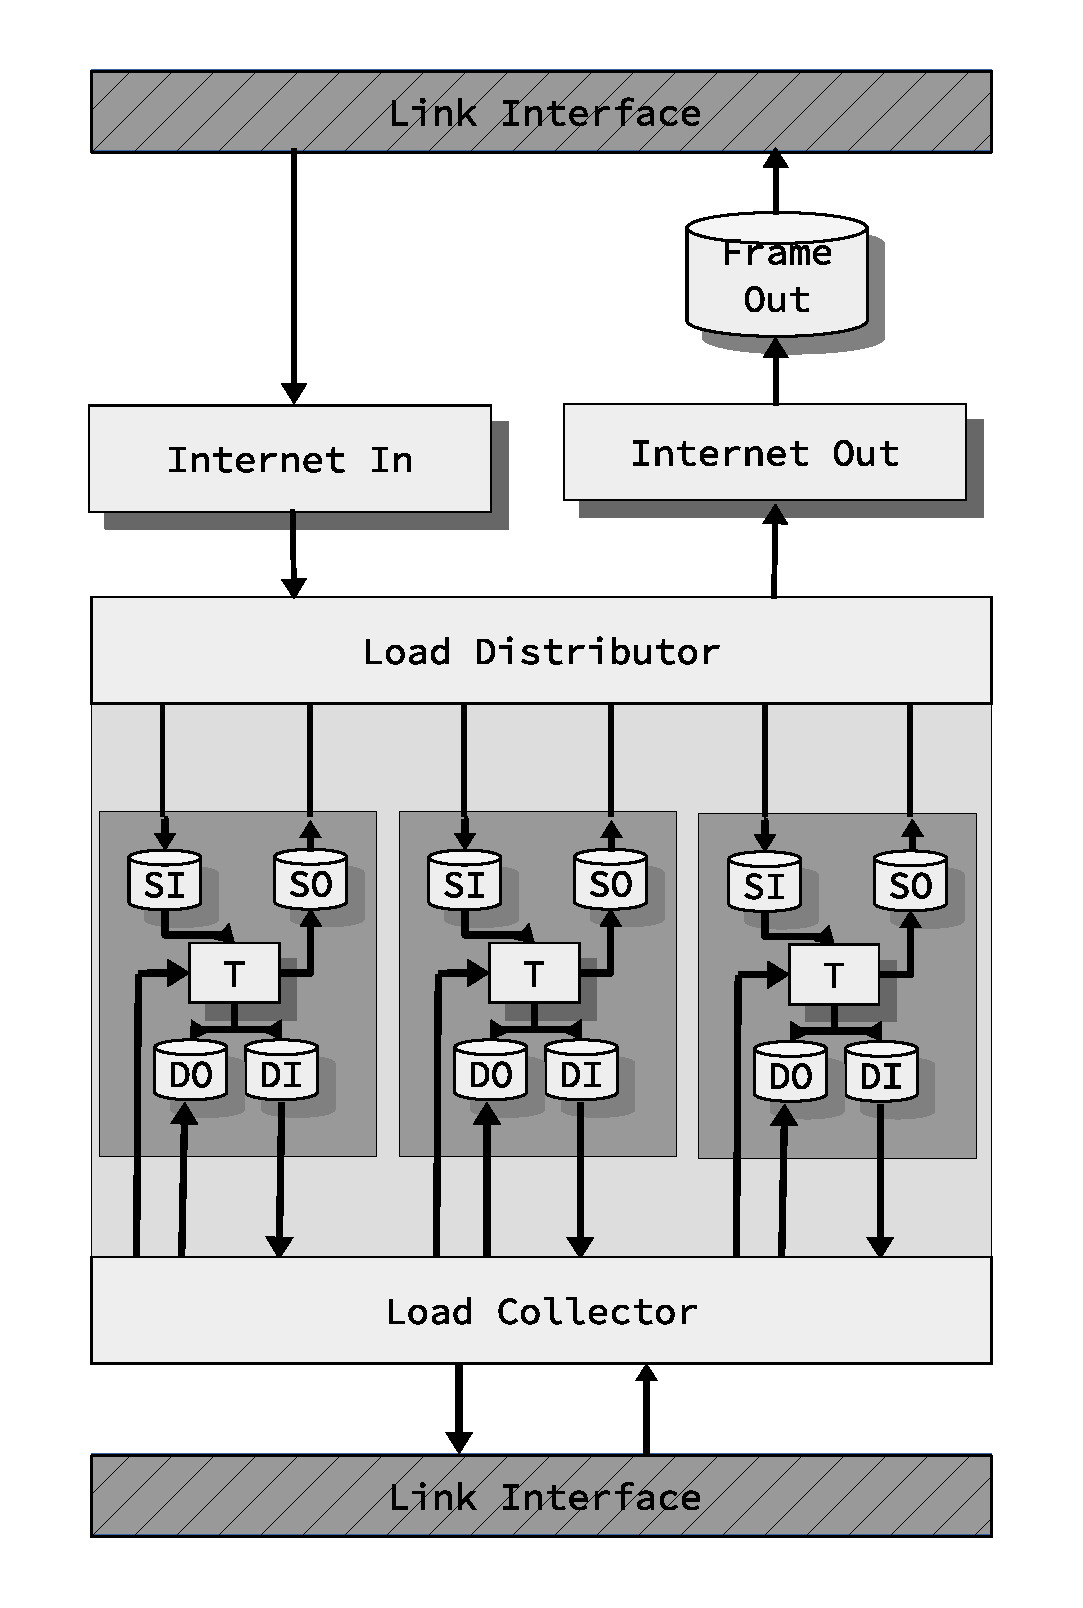
\includegraphics[scale=0.25]{../thesis/discussion/design_stacked.eps}
\end{figure}
\end{column}
\end{columns}

\end{frame}


\begin{frame}
\begin{columns}
\begin{column}{0.5\textwidth}
Usability

\end{column}

\begin{column}{0.5\textwidth}
SOMETHING
\end{column}
\end{columns}
\end{frame}

\begin{frame}
\begin{columns}
\begin{column}{0.5\textwidth}
Using C\#
\end{column}

\begin{column}{0.5\textwidth}
State modelling\\
Simulation\\
Concurrency
\end{column}
\end{columns}
\end{frame}

\section{Conclusion}
\begin{frame}
  \frametitle{Conclusion}

\begin{itemize}
\item The design underwent many alternations, but the final layered design
has proven to work great
\item In 1.83 mio. simulated clock cycles, all of 17283 packets were handled
correctly

\item Errors in the outgoing packets, but they should be easily fixable

\item SME was of great help for the implementation, albeit with a few errors and
bugs

\end{itemize}

\end{frame}
